\usecaseristoratore{Visualizzazione lista ordinazioni}
\label{usecase:Visualizzazione lista ordinazioni}

\begin{figure}[h]
	\centering
	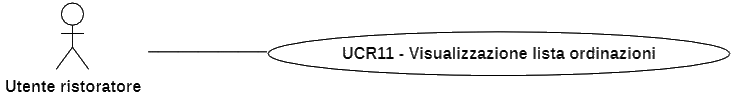
\includegraphics[width=0.9\textwidth]{./uml/UCR11.png} 
	\caption{Visualizzazione lista ordinazioni}
	\label{fig:UCR11}
  \end{figure}

\begin{itemize}
	\item \textbf{Attore principale:} Utente ristoratore.

	\item \textbf{Precondizione:} L'Utente ristoratore visualizza il dettaglio di una prenotazione (vedi \autoref{usecase:Visualizza dettaglio lista prenotazioni}).

	\item \textbf{Postcondizione:} L'Utente ristoratore visualizza tutte le
	      ordinazioni presenti all'interno della prenotazione.

	\item \textbf{Scenario principale:}
	      \begin{enumerate}
		      \item Il Sistema mostra al ristoratore la lista delle ordinazioni fatte dai clienti.

				\item Per ogni ordinazione il Sistema mostra:
					\begin{itemize}
						\item Il nome dell'utente che ha effettuato
							l'ordinazione;
						\item Il costo dell'ordinazione dell'utente;
						\item I piatti che compongono l'ordinazione:
							\begin{itemize}
								\item Il nome del piatto;
								\item Il prezzo del piatto;
								\item Lo stato di pagamento del piatto;
								\item Gli ingredienti rimossi dal piatto;
							\end{itemize}
					\end{itemize}
	      \end{enumerate}
\end{itemize}

